% Supercapacitor results
    \subsection{Comportement du système}

Les comportements du système ont ensuite été étudiés. Comme nous l'avons évoqué précédemment, nous souhaitons étudier la distribution des charges au sein des électrodes et les phénomènes d'adsorption des ions.

Pour ce faire, nous avons imaginé trois systèmes : un système chargé à \qty{4.0}{\volt}, un système non chargé, et un système chargé à \qty{4.0}{\volt} comportant un défaut sur une des électrodes. Le défaut choisi a été un atome de carbone manquant.\\
Pour chacun d'eux, deux simulations ont été effectuées : pour un nombre arbitraire d'ions (\num{10} paires d'ions entre les électrodes), et pour une concentration d'\qty{1}{\mole \per \liter} (soit \num{2} paires d'ions entre les électrodes).

Chacune de ces simulations a suivi le déroulement de la \autoref{sec:deroulement_simulations}, c'est-à-dire :
\begin{itemize}
    \item une minimisation à \qty{0}{\kelvin}
    \item une relaxation de \qty{0.01}{\nano \second} à \qty{300}{\kelvin} et \qty{1}{\atm}
    \item une stabilisation de \qty{0.01}{\nano \second} à \qty{300}{\kelvin} et \qty{1}{\atm}
    \item la simulation principale à \qty{300}{\kelvin} et \qty{1}{\atm} pour \qty{1}{\nano \second}
\end{itemize}

Les grandeurs thermodynamiques lors des différentes étapes de simulation sont présentées aux \autoref{fig:relaxation_thermo} et \ref{fig:main_thermo}. À partir de ces graphes, nous estimons que l'équilibre est atteint pour les trois systèmes à partir de \num{4000000} d'itérations soit \qty{0.4}{\nano \second} : en effet, puisque la température est contrôlée nous ne pouvons nous reposer sur sa valeur comme indication de l'équilibre ; De plus, puisque l'énergie potentielle des systèmes dépend de s'ils sont chargés ou non cette grandeur n'est pas utile non plus ; Ainsi nous nous reposons sur la pression pour nous indiquer l'équilibre du système.

\begin{figure}[h!]
    \centering
    \begin{subfigure}[t]{.49 \textwidth}
        \centering
        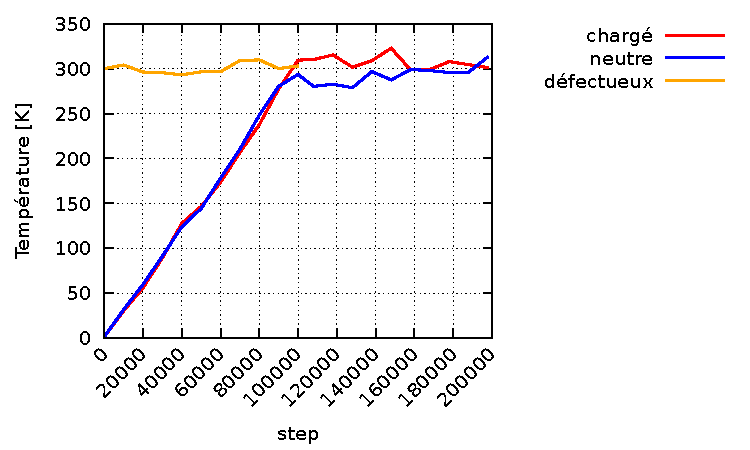
\includegraphics[width = \textwidth]{relaxation_temp.pdf}
        \caption{Température}
    \end{subfigure}%
    ~
    \begin{subfigure}[t]{.49 \textwidth}
        \centering
        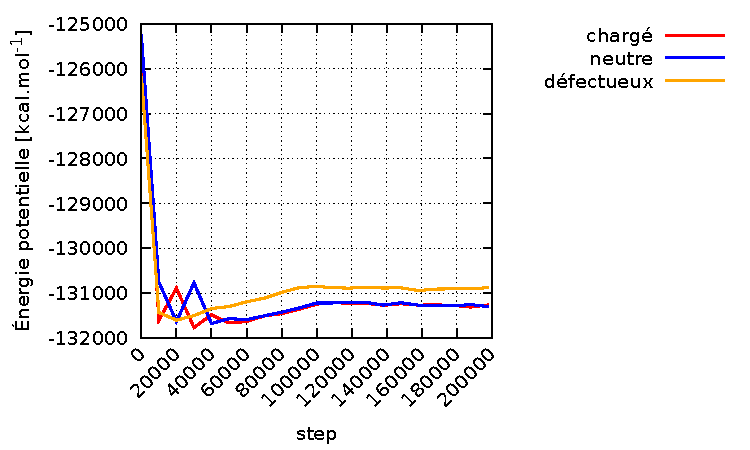
\includegraphics[width = \textwidth]{relaxation_epot.pdf}
        \caption{Énergie potentielle par atome}
    \end{subfigure}
    \begin{subfigure}[t]{.49 \textwidth}
        \centering
        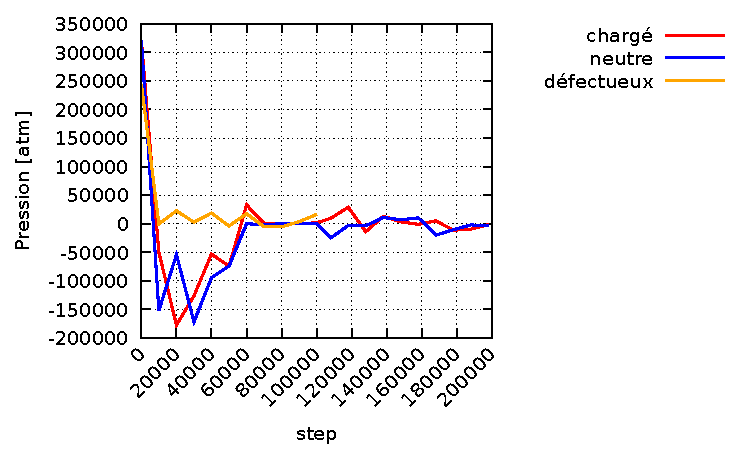
\includegraphics[width = \textwidth]{relaxation_press.pdf}
        \caption{Pression}
    \end{subfigure}
    \caption{Grandeurs thermodynamiques au cours de la relaxation et stabilisation}
    \label{fig:relaxation_thermo}
\end{figure}

\begin{figure}[h!]
    \centering
    \begin{subfigure}[t]{.49 \textwidth}
        \centering
        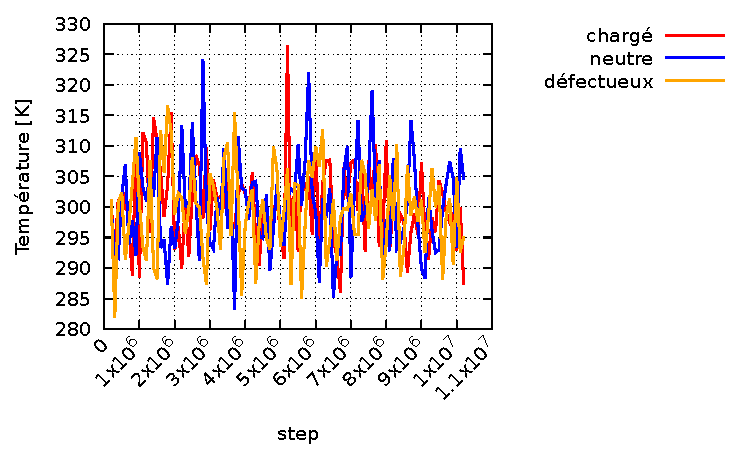
\includegraphics[width = \textwidth]{main_temp.pdf}
        \caption{Température}
    \end{subfigure}%
    ~
    \begin{subfigure}[t]{.49 \textwidth}
        \centering
        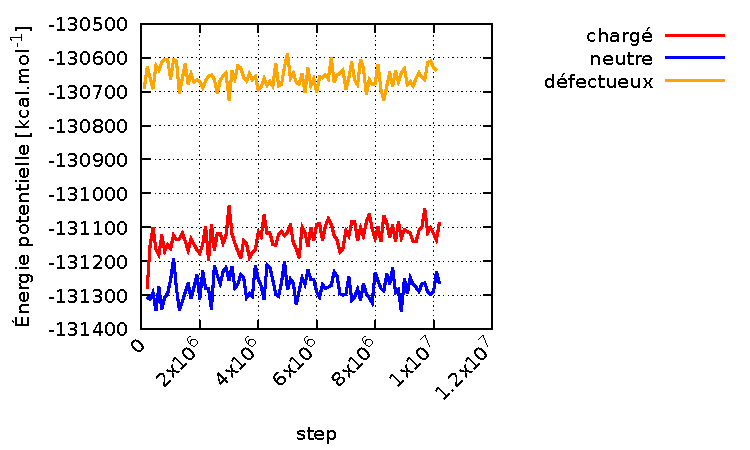
\includegraphics[width = \textwidth]{main_epot.pdf}
        \caption{Énergie potentielle par atome}
    \end{subfigure}
    \begin{subfigure}[t]{.49 \textwidth}
        \centering
        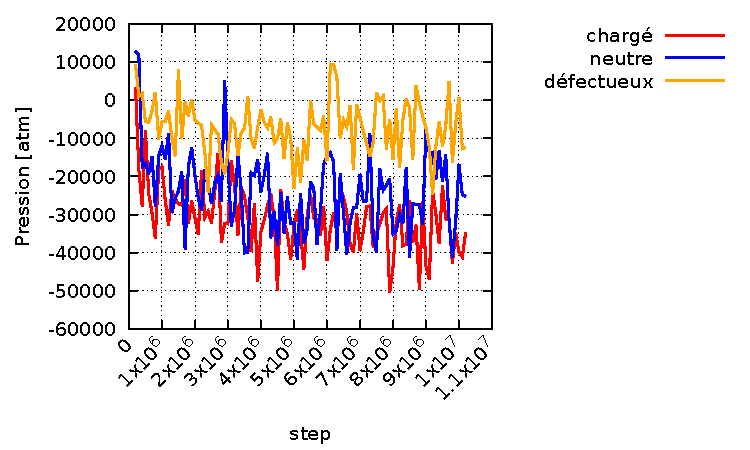
\includegraphics[width = \textwidth]{main_press.pdf}
        \caption{Pression}
    \end{subfigure}
    \caption{Grandeurs thermodynamiques au cours de la simulation principale}
    \label{fig:main_thermo}
\end{figure}

% Charge distribution on the electrode
    \subsubsection{Distribution des charges sur les électrodes}

La distribution des charges sur les électrodes est mesurée par la moyenne des charges au sein de certains groupes d'atomes. Ceux-ci sont : les atomes de carbone composant les couches extérieures des électrodes, les atomes des couches intérieures, les atomes voisins du défaut.\\
La \autoref{fig:charges_groupes} présente les différents graphes obtenus pour cette mesure pour les différents systèmes, les \autoref{fig:comparaison_ch-sc-defected} et \ref{fig:comparaison_ch-sc-neutral} présentent des comparaisons entre les systèmes, et le \autoref{tab:comparaison_charges} résume les moyennes des charges suivant le groupe d'atomes de carbone.

\begin{figure}[h!]
    \centering
    \begin{subfigure}[t]{.49 \textwidth}
        \centering
        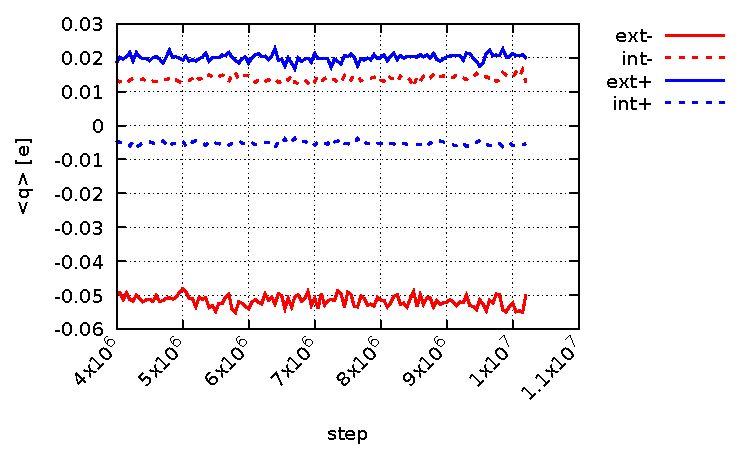
\includegraphics[width = \textwidth]{ch-sc_q-1.pdf}
        \caption{Pour le système chargé}
        \label{fig:charges_groupes_ch-sc}
    \end{subfigure}%
    ~
    \begin{subfigure}[t]{.49 \textwidth}
        \centering
        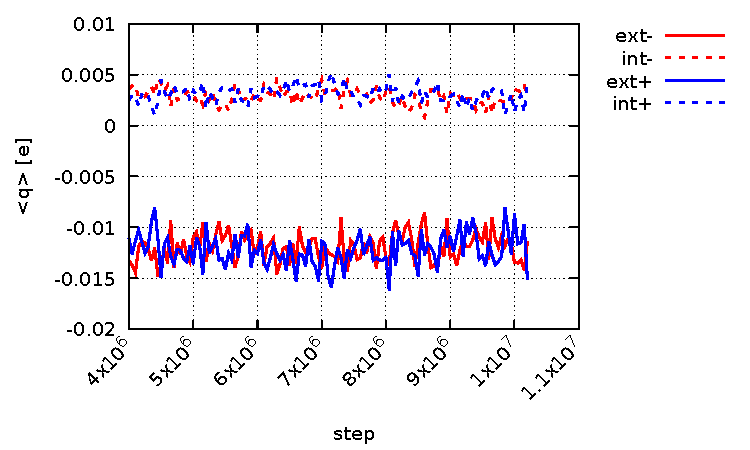
\includegraphics[width = \textwidth]{neutral_q-1.pdf}
        \caption{Pour le système non chargé}
        \label{fig:charges_groupes_neutral}
    \end{subfigure}
    
    \begin{subfigure}[t]{.49 \textwidth}
        \centering
        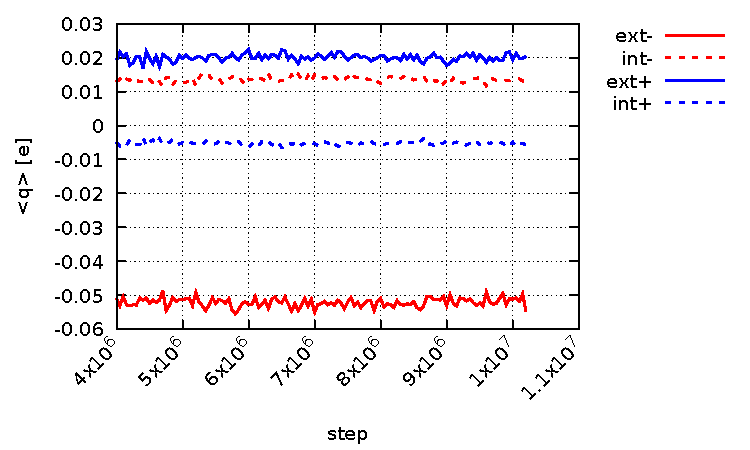
\includegraphics[width = \textwidth]{defected_q-1.pdf}
        \caption{Pour le système défectueux}
        \label{fig:charges_groupes_defected}
    \end{subfigure}

    \caption{Distribution des charges par groupes d'atomes. Les groupes d'atomes communs sont les carbones des couches intérieures et extérieures des deux électrodes ; Et pour le système défectueux il y a les atomes voisins du défaut}
    \label{fig:charges_groupes}
\end{figure}

\begin{figure}[h!]
    \centering
    \begin{subfigure}[t]{.49 \textwidth}
        \centering
        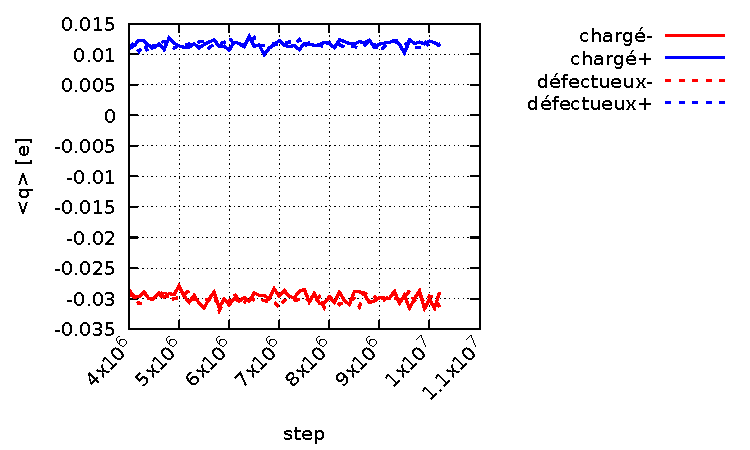
\includegraphics[width = \textwidth]{q_ch-sc-defected.pdf}
        \caption{Pour toutes les couches}
    \end{subfigure}%
    ~
    \begin{subfigure}[t]{.49 \textwidth}
        \centering
        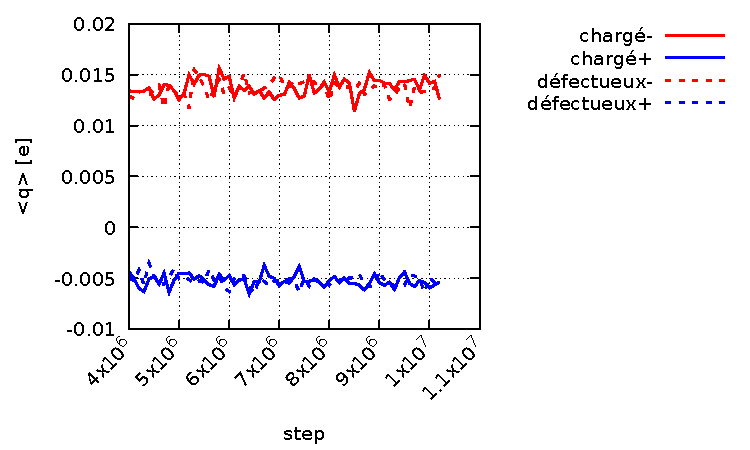
\includegraphics[width = \textwidth]{q_ch-sc-defected-inn.pdf}
        \caption{Pour les couches intérieures}
    \end{subfigure}

    \begin{subfigure}[t]{.49 \textwidth}
        \centering
        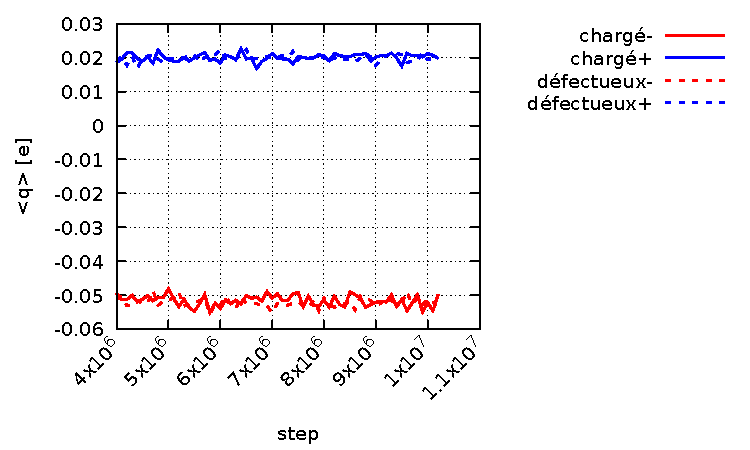
\includegraphics[width = \textwidth]{q_ch-sc-defected-out.pdf}
        \caption{Pour les couches extérieures}
    \end{subfigure}
    \caption{Comparaison des charges entre le système chargé et le système défectueux}
    \label{fig:comparaison_ch-sc-defected}
\end{figure}

\begin{figure}[h!]
    \centering
    \begin{subfigure}[t]{.49 \textwidth}
        \centering
        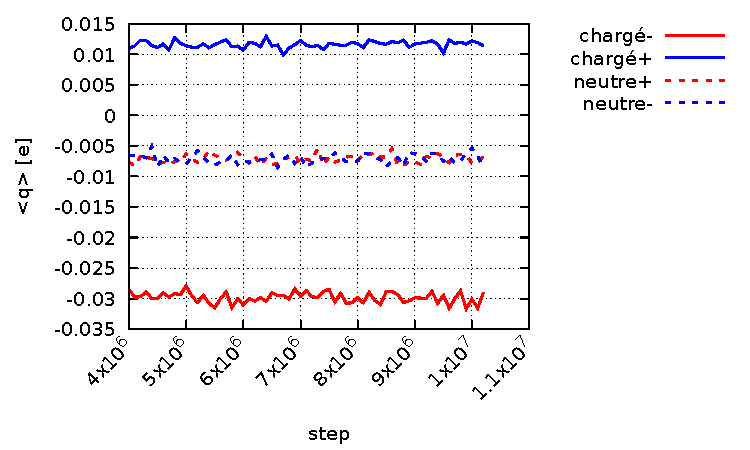
\includegraphics[width = \textwidth]{q_ch-sc-neutral.pdf}
        \caption{Pour toutes les couches}
    \end{subfigure}%
    ~
    \begin{subfigure}[t]{.49 \textwidth}
        \centering
        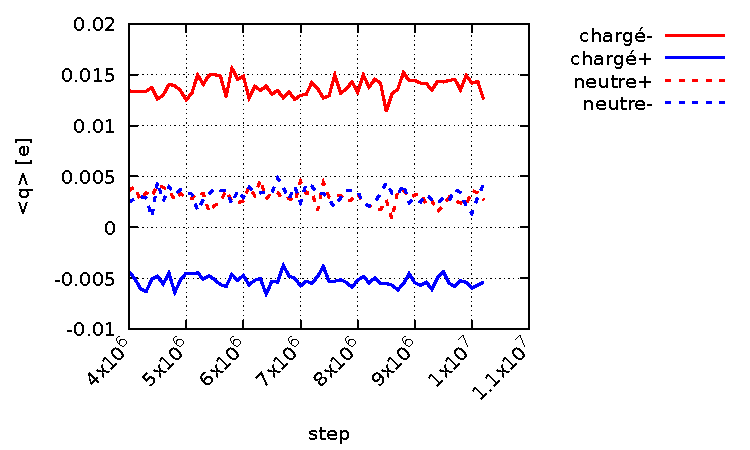
\includegraphics[width = \textwidth]{q_ch-sc-neutral-inn.pdf}
        \caption{Pour les couches intérieures}
    \end{subfigure}

    \begin{subfigure}[t]{.49 \textwidth}
        \centering
        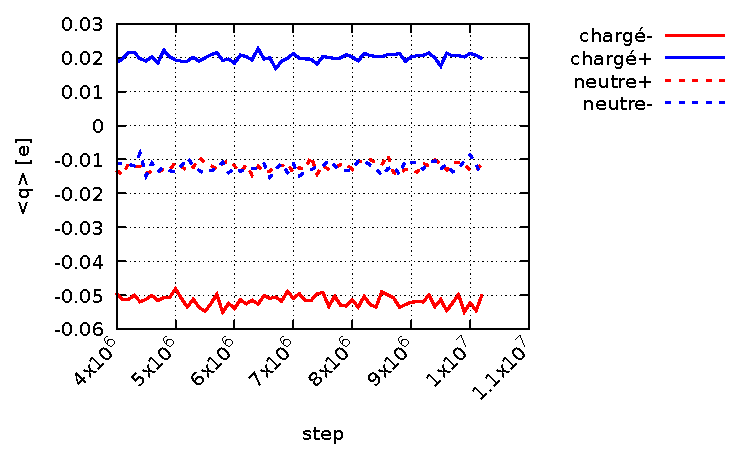
\includegraphics[width = \textwidth]{q_ch-sc-neutral-out.pdf}
        \caption{Pour les couches extérieures}
    \end{subfigure}
    \caption{Comparaison des charges entre le système chargé et le système non chargé}
    \label{fig:comparaison_ch-sc-neutral}
\end{figure}

\begin{table}[h!]
    \centering
    \begin{tabular}{c | c | c || c}
        \hline
        Système &Électrode &Couches &Moyenne des charges [\unit{\e}]\\
        \hline
        chargé &négative &toutes &\num{-0.0299}\\
         & &intérieures &\num{0.0138}\\
         & &extérieures &\num{-0.0517}\\
         &positive &toutes &\num{0.0116}\\
         & &intérieures &\num{-0.0052}\\
         & &extérieures &\num{0.0200}\\
        \hline
        neutre &négative &toutes &\num{-0.0070}\\
         & &intérieures &\num{0.0031}\\
         & &extérieures &\num{-0.0121}\\
        &positive &toutes &\num{-0.0071}\\
         & &intérieures &\num{0.0028}\\
         & &extérieures &\num{-0.0119}\\ 
        \hline
        défectueux &négative &toutes &\num{-0.0300}\\
         & &intérieures &\num{0.0135}\\
         & &extérieures &\num{-0.0519}\\
         &positive &toutes &\num{0.0116}\\
         & &intérieures &\num{-0.0052}\\
         & &extérieures &\num{0.0200}\\
        \hline
    \end{tabular}
    \caption{Tableau récapitulatif des moyennes des charges en fonction du groupe de carbone}
    \label{tab:comparaison_charges}
\end{table}

\clearpage

\textbf{Observations}\\
Pour les systèmes chargés (\autoref{fig:charges_groupes_ch-sc} et \ref{fig:charges_groupes_defected}, et \autoref{tab:comparaison_charges}), il semble que les charges des électrodes soient situées plutôt sur leurs couches extérieures : pour l'électrode négative les couches extérieures sont chargées négativement, tandis que pour l'électrode positive elles sont chargées positivement.

Pour le système neutre (\autoref{fig:charges_groupes_neutral}, et \autoref{tab:comparaison_charges}), nous pouvons voir un décalage de charges entre les couches : les couches extérieures sont chargées négativement tandis que les couches intérieures sont chargées positivement, de plus les couches extérieures sont plus chargées que les couches intérieures. Mais malgré ces décalages, les moyennes des charges sont quasimment les mêmes pour les deux électrodes et leurs couches respectives.

En comparant les systèmes chargés (\autoref{fig:comparaison_ch-sc-defected}, et \autoref{tab:comparaison_charges}), nous voyons que les charges des deux systèmes sont quasimment les mêmes pour les deux électrodes et leurs couches séparément.

En comparant les systèmes chargés au système non chargé (\autoref{fig:comparaison_ch-sc-neutral}, et \autoref{tab:comparaison_charges}), nous pouvons voir que pour les systèmes chargés l'écart de charges entre les couches intérieures et extérieures est plus grand pour l'électrode négative que pour l'électrode positive (\qtyrange[range-units = single]{125}{135}{\percent}) par rapport aux valeurs du système non chargé.

\textbf{Interprétations}\\
La différence de charges entre les couches extérieures et intérieures peut avoir deux raisons :
\begin{itemize}
    \item La polarisation du système a pour conséquence d'attirer les charges d'une électrode vers l'autre ; Puisque le système est périodique selon la direction orthogonale aux surfaces des électrodes (selon la direction $[Oz)$), les charges d'une électrode sont attirées vers l'électrode opposée et son image périodique, c'est-à-dire vers les couches extérieures
    \item Au commencement de l'analyse des données (à partir de \qty{0.4}{\nano \second}), la double couche électrochimique (\edl{}) est déjà formée et les charges de chaque électrode sont concentrées à leurs interfaces avec l'électrolyte
\end{itemize}

Quant au décalage de charges entre les couches du système non chargé, puisqu'il n'existe pas de différence de potentiel entre les électrodes il est possible que ce phénomène ne soit qu'une conséquence de l'interface entre l'électrode et l'électrolyte.

L'absence de différences notables entre les charges des systèmes chargés nous laisse penser que la présence du défaut n'influence pas la charge du système dans sa globalité.

Pour les écarts de charges entre les couches intérieures et extérieures du système chargé par rapport aux valeurs du système neutre, il n'y a pas de raison apparente. Cependant, le fait que pour les trois groupes d'atomes (couches intérieures, extérieures, et intégralité de l'électrode) il y ait un rapport d'environ $\num{1.25}\sim \num{1.35}$ nous laisse penser qu'il existe une raison sous-jacente et non évidente.

% Ions adsorption/displacement
    \subsubsection{Adsorption et déplacements des ions}

L'adsorption des ions est mesurée par deux grandeurs : la densité numérique d'ions dans l'électrolyte, et la fonction de ditribution radiale entre les ions et les carbones des électrodes.

Les \autoref{fig:densite} et \ref{fig:comparaison_densite} présentent la densité numérique d'ions dans l'électrolyte en fonction de la direction $[Oz)$ (correspondant à la direction orthogonale aux surfaces des électrodes) au début de l'analyse (à \qty{0.4}{\nano \second}) et à la fin (à \qty{1.0}{\nano \second}) pour les systèmes chargés et le système neutre.\\
Quant aux \autoref{fig:rdf_ch-sc-neutral} et \ref{fig:rdf_ch-sc-defected}, elles montrent les fonctions de distribution radiale des ions sodium et hydroxyde de l'électrolyte par rapport aux carbones des deux électrodes des trois systèmes.

\begin{figure}[h!]
    \centering
    \begin{subfigure}[t]{.49 \textwidth}
        \centering
        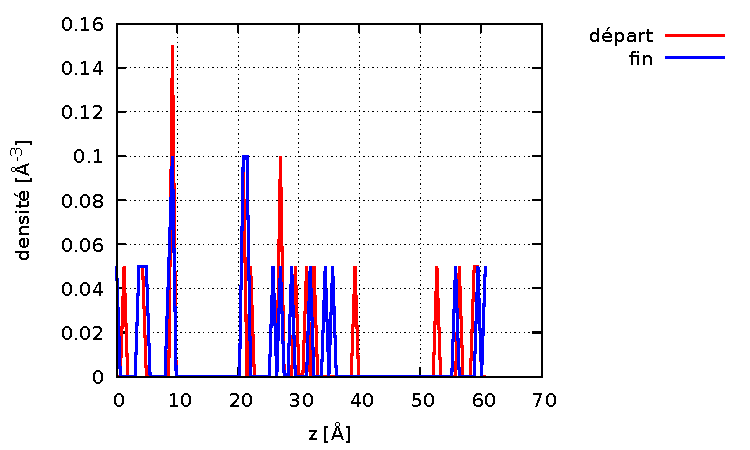
\includegraphics[width = \textwidth]{ch-sc_density.pdf}
        \caption{Pour le système chargé}
    \end{subfigure}%
    ~
    \begin{subfigure}[t]{.49 \textwidth}
        \centering
        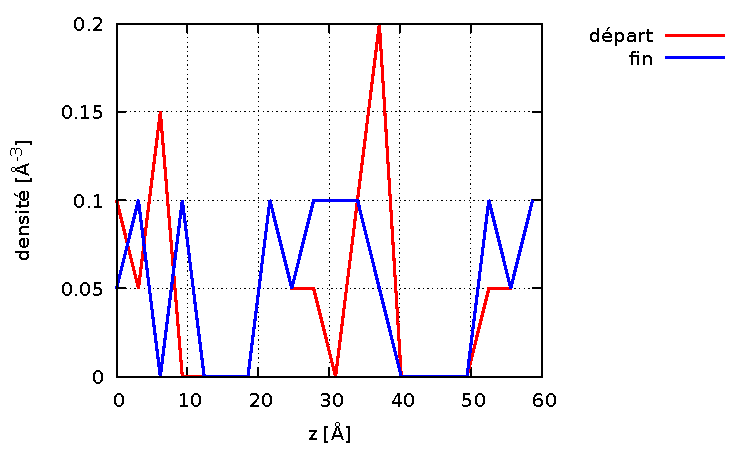
\includegraphics[width = \textwidth]{neutral_density.pdf}
        \caption{Pour le système non chargé}
    \end{subfigure}

    \begin{subfigure}[t]{.49 \textwidth}
        \centering
        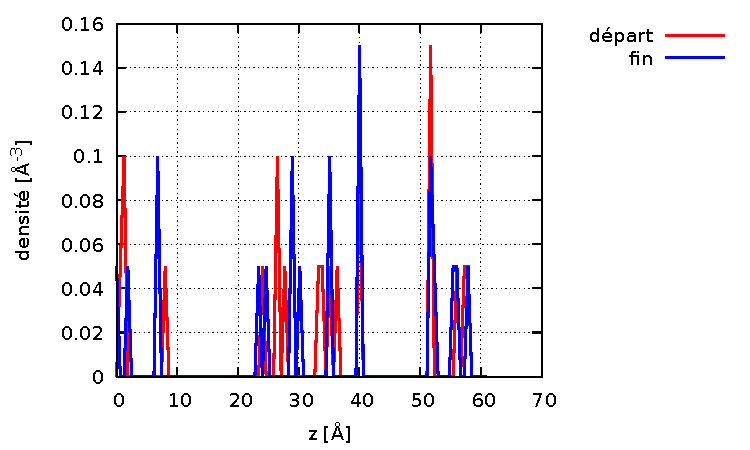
\includegraphics[width = \textwidth]{defected_density.pdf}
        \caption{Pour le système défectueux}
    \end{subfigure}
    \caption{Densité numérique d'ions sodium dans l'électrolyte}
    \label{fig:densite}
\end{figure}

\begin{figure}[h!]
    \centering
    \begin{subfigure}[t]{.49 \textwidth}
        \centering
        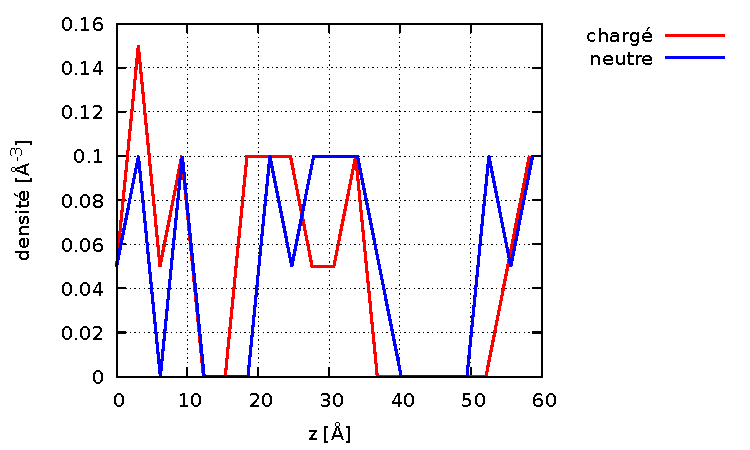
\includegraphics[width = \textwidth]{density_ch-sc-neutral.pdf}
        \caption{Entre le système chargé et le système neutre}
    \end{subfigure}%
    ~
    \begin{subfigure}[t]{.49 \textwidth}
        \centering
        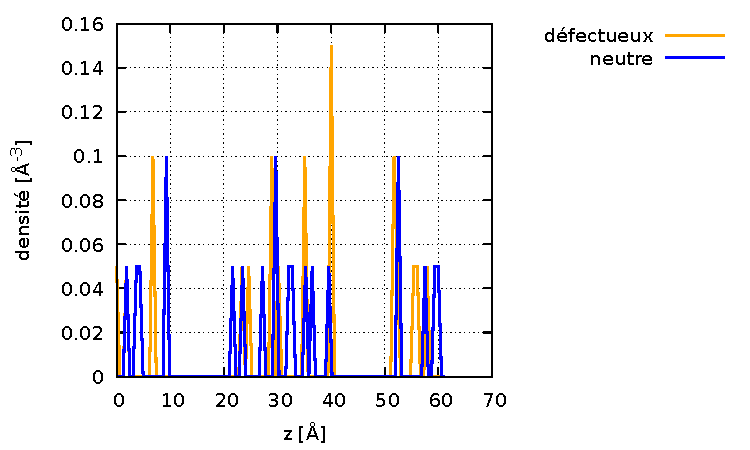
\includegraphics[width = \textwidth]{density_defected-neutral.pdf}
        \caption{Entre le système défectueux et le système neutre}
    \end{subfigure}
    \caption{Comparaisons des densités numériques finales}
    \label{fig:comparaison_densite}
\end{figure}

\begin{figure}[h!]
    \centering
    \begin{subfigure}[t]{.49 \textwidth}
        \centering
        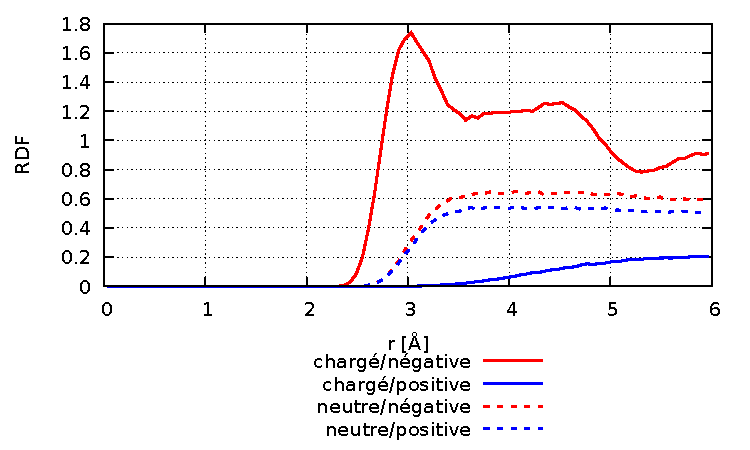
\includegraphics[width = \textwidth]{rdf_ch-sc-neutral-Na.pdf}
        \caption{Pour les ions sodium par rapport à l'électrode négative}
    \end{subfigure}%
    ~
    \begin{subfigure}[t]{.49 \textwidth}
        \centering
        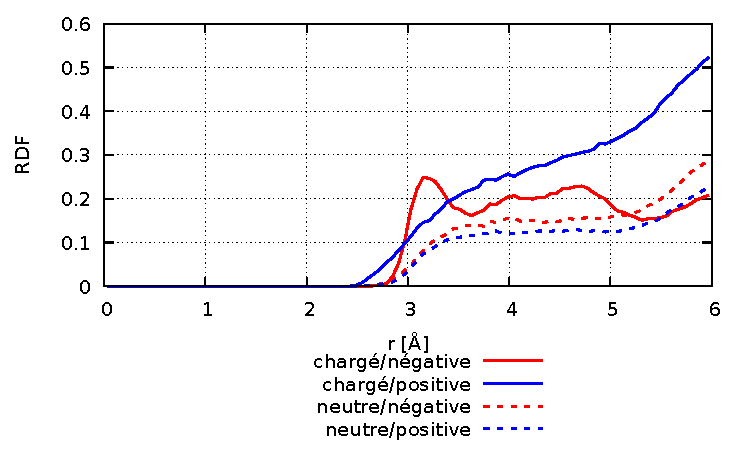
\includegraphics[width = \textwidth]{rdf_ch-sc-neutral-OH.pdf}
        \caption{Pour les ions hydroxyde par rapport à l'électrode positive}
    \end{subfigure}

    \begin{subfigure}[t]{.49 \textwidth}
        \centering
        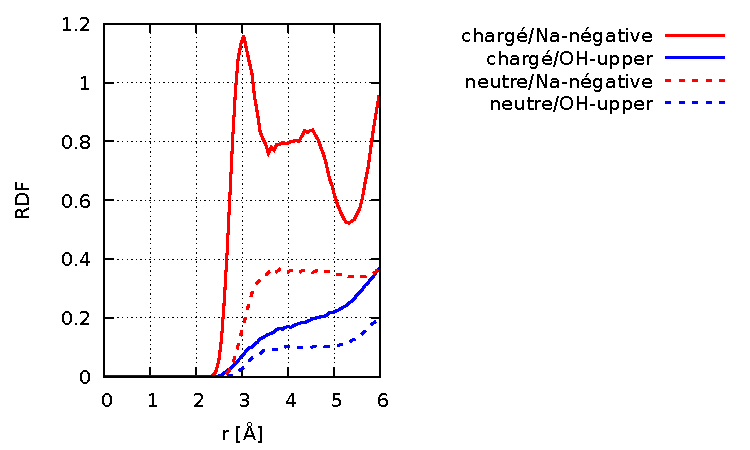
\includegraphics[width = \textwidth]{rdf_ch-sc-neutral-NaOH.pdf}
        \caption{Pour les tous ions, par rapport à leurs électrodes respectives}
    \end{subfigure}
    \caption{Comparaison des fonctions de distribution radiale des ions par rapport aux carbones des électrodes entre le système chargé et le système neutre}
    \label{fig:rdf_ch-sc-neutral}
\end{figure}

\begin{figure}[h!]
    \centering
    \begin{subfigure}[t]{.49 \textwidth}
        \centering
        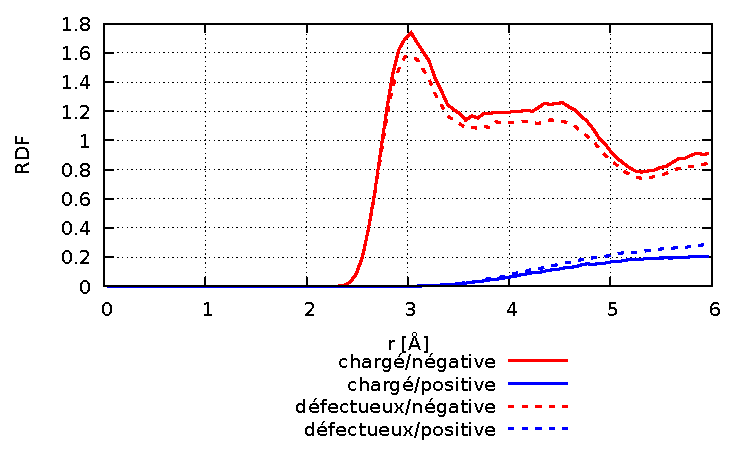
\includegraphics[width = \textwidth]{rdf_ch-sc-defected-Na.pdf}
        \caption{Pour les ions sodium par rapport à l'électrode négative}
    \end{subfigure}%
    ~
    \begin{subfigure}[t]{.49 \textwidth}
        \centering
        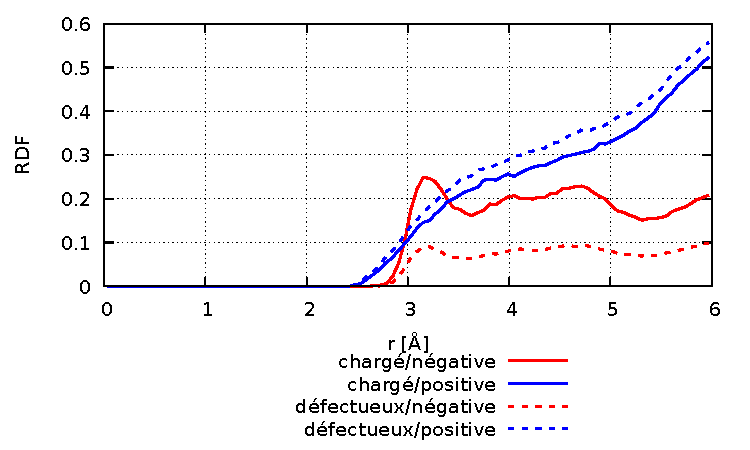
\includegraphics[width = \textwidth]{rdf_ch-sc-defected-OH.pdf}
        \caption{Pour les ions hydroxyde par rapport à l'électrode positive}
    \end{subfigure}

    \begin{subfigure}[t]{.49 \textwidth}
        \centering
        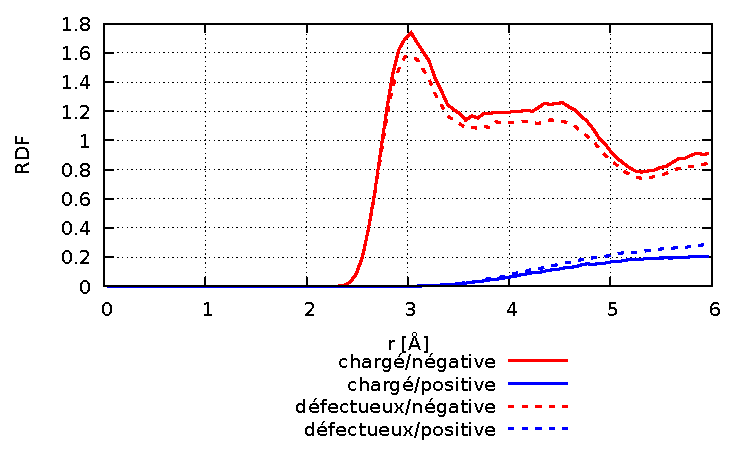
\includegraphics[width = \textwidth, draft]{rdf_ch-sc-defected-Na.pdf}
        \caption{Pour les ions sodium par rapport à l'électrode négative en extrayant les carbones voisins du défaut}
    \end{subfigure}%
    ~
    \begin{subfigure}[t]{.49 \textwidth}
        \centering
        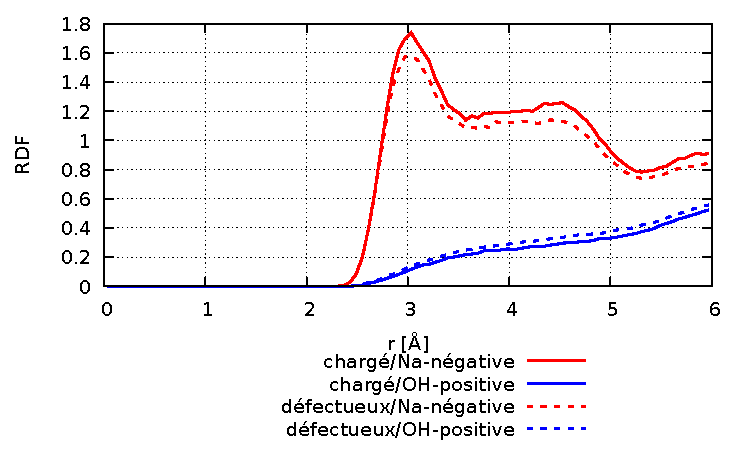
\includegraphics[width = \textwidth]{rdf_ch-sc-defected-NaOH.pdf}
        \caption{Pour tous les ions, par rapport à leurs électrodes respectives}
    \end{subfigure}
    \caption{Comparaison des fonctions de distribution radiale des ions par rapport aux carbones des électrodes entre le système chargé et le système défectueux}
    \label{fig:rdf_ch-sc-defected}
\end{figure}

\clearpage
\textbf{Observations}\\
BLABLA

\textbf{Interprétations}\\
BLABLA
